\documentclass[a4paper, 12pt]{article} % Adicionado tamanho do papel e fonte maior (12pt)
\usepackage[utf8]{inputenc}
\usepackage{array}
% --- Configurações de Margem ---
\usepackage[a4paper, margin=2.5cm]{geometry} % É AQUI QUE A MÁGICA ACONTECE! 
% Se o professor exigir ABNT, troque a linha acima por:
% \usepackage[a4paper, left=3cm, right=2cm, top=3cm, bottom=2cm]{geometry}
\usepackage{float}
\usepackage{csquotes}
% --- Idioma e Codificação ---
\usepackage[T1]{fontenc}
\usepackage[utf8]{inputenc} % Garante que acentos funcionem (opcional nas versões mais recentes, mas seguro)
\usepackage[portuguese]{babel} % Hifenização correta e tradução (ex: "Abstract" vira "Resumo")
\usepackage{tabularx}
% --- Pacotes Úteis para Relatórios ---
\usepackage{graphicx} % Para inserção de imagens (o que você já tinha)
\usepackage{hyperref} % Deixa o sumário e as URLs clicáveis
\usepackage{url}
\usepackage{microtype} % Melhora drasticamente a justificação do texto (evita buracos brancos)
\usepackage{indentfirst} % Indenta o primeiro parágrafo de cada seção (padrão do português)
\usepackage{amsfonts}
\usepackage[backend=biber, style=abnt]{biblatex} % style=abnt para ABNT, ou style=ieee
\addbibresource{./sbc-template.bib}
\usepackage{listings}
\usepackage{xcolor}
\usepackage{sbc-template}

% Configuração básica para parecer com o seu exemplo
\lstset{
  basicstyle=\ttfamily\small,
  backgroundcolor=\color{gray!10},
  frame=single,
  breaklines=true
}

% --- Dados da Capa ---
\title{\textbf{EP2 de Bancos de dados}}
\author{\small\textit{ Luiz Fernando de Freitas Fernandes -- 13671678}}


\newcommand{\code}[1]{\texttt{#1}}
\begin{document}

\maketitle

% Certifique-se de que os seguintes pacotes estejam no preâmbulo do seu documento (antes do \begin{document}):
% \usepackage{graphicx}
% \usepackage{amsmath}
% \usepackage{booktabs}
% \usepackage{float}

\section{Algoritmos de Vizinhos Mais Próximos Aproximados (ANN)}

Algoritmos ANN podem ser pensados como buscas de vizinhos mais próximos (k-NN) que não necessariamente retornam esse vizinho mais próximo, mas sim algum ponto dentro de uma margem de erro em volta dele. Mais formalmente, seja $D: \mathbb{R}^d \times \mathbb{R}^d \rightarrow \mathbb{R}$ uma métrica de distância e $P \subset \mathbb{R}^d$ um conjunto de $n$ pontos. Um algoritmo para um problema $\epsilon$-ANN recebe como entrada um ponto $q \in \mathbb{R}^d$ e devolve um ponto $p \in P$ tal que, para todo $p' \in P$, $D(p, q) \leq (1 + \epsilon)D(p', q)$. Alguns algoritmos desse tipo encontraram sucesso em mitigar a maldição da dimensionalidade, os principais sendo o \textit{Hierarchical Navigable Small World} e o \textit{Inverted File Index} com quantização de produto.

\subsection{\textit{Hierarchical Navigable Small World} (HNSW)}

o HNSW é um aperfeiçoamento de outro algoritmo ANN chamado \textit{Navigable Small World} (NSW), que por sua vez usa o conceito de grafos navegáveis para tentar resolver o problema eficientemente.

\subsubsection{Conceitos}

Um \textit{grafo de proximidade} $G$ é um grafo direcionado onde seus vértices representam um subconjunto de pontos de um espaço métrico e as arestas são tais que k-NN pode ser resolvido de forma gulosa. Isso significa que, dado um ponto $q$ desse espaço, o seguinte procedimento sempre termina e devolve o vértice de $G$ mais próximo de $q$: começando em um vértice arbitrário $p$, itera-se por todos os seus vizinhos e, se nenhum deles tem distância estritamente menor que a distância entre $p$ e $q$, $p$ é retornado, caso contrário o vizinho com a menor distância é selecionado e o processo se repete a partir dele.

Um \textit{grafo navegável} é um grafo de proximidade no qual o algoritmo guloso termina em tempo logarítmico ou polilogarítmico em relação ao tamanho do grafo. 

\subsubsection{Funcionamento}

O NSW organiza os índices dos vetores gerando uma aproximação de um grafo navegável. Primeiramente, é definido um limite $M$ do número de vizinhos que um vértice pode ter, e depois cada vértice é inserido em ordem aleatória e ligado aos $M$ vértices mais próximos que já foram inseridos. Infelizmente, o algoritmo guloso apresenta performance polilogarítmica, limitando sua utilidade.

Visando melhorar essa performance, o HNSW junta o NSW com a ideia de \textit{skip lists}: é implementado uma aproximação de um grafo navegável multi-camadas no qual a camada base tem todos os vértices e cada vértice tem uma chance de aparecer na próxima camada que cai exponencialmente. 

\begin{figure}[ht]
    \centering
    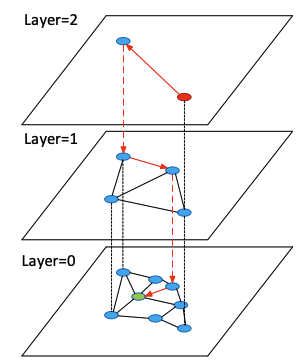
\includegraphics[width=0.5\linewidth]{hnsw_layers.png}
    \caption{Exemplo de execução da busca em um HNSW. O algoritmo guloso começa na camada mais alta, acha o ponto aproximadamente ótimo dessa camada e repete o processo na camada de baixo, até chegar na última camada que tem todos os vértices.}
    \label{fig:placeholder}
\end{figure}

A inserção possui 3 parâmetros principais: o ponto $q$ que será inserido, o limite $M$ de vizinhos por vértice em uma camada, e o limite $efConstruction$ de potenciais vizinhos de $q$. Na inserção de um novo vértice $q$, primeiro é sorteado $l$, que é a camada mais alta na qual $q$ aparecerá. Em seguida, o algoritmo guloso é usado na camada mais superior para achar o vértice dela mais próximo de $q$, e é usado novamente a partir desse vértice achado no passo anterior, porém uma camada abaixo. Isso se repete até a camada $l$ ser alcançada, a partir da qual o procedimento do NSW é feito até a camada base, porém considerando apenas $efConstruction$ vértices por camada.

A busca pelo vértice mais próximo de um ponto $q$ é similar à inserção: o algoritmo guloso começa de um vértice arbitrário da camada mais elevada, acha o vértice $p$ dessa camada mais próximo de $q$, e reinicia o processo a partir de $p$ mas uma camada abaixo, até chegar na camada base.

É importante notar que, sendo $p=\exp(-m_L)$, para algum $m_L$, a probabilidade de um vértice aparecer na camada acima da atual, a busca nessa camada sempre acaba antes de chegar em alguns desses vértices. Isso vem das propriedades de grafos de proximidade, já que cada passo do algoritmo guloso necessariamente diminui a distância entre o ponto atual e o desejado, mas se durante a execução do algoritmo um vértice que está na camada superior é visitado, isso significa que esse vértice tem uma distância menor do que o vértice usado para descer dessa camada superior, mas esse era para ser o ótimo da camada, gerando uma contradição. Assim, a probabilidade do algoritmo guloso descer de camada depois de $k$ passos é $p^k=\exp(-km_L)$, portanto o número de passos esperado por camada é limitado pela soma da progressão geométrica em $k$, que independe do tamanho do grafo ou do número de dimensões dos vetores. Visto que o número de vizinhos checados por passo também é limitado por uma constante ($M$), o tempo de execução por camada é assintoticamente constante e, como o número de camadas esperado é $O(\log(N))$ (já que depende exponencialmente de $p$), o tempo de execução esperado da busca é $O(\log(N))$, mostrando que realmente em relação ao tempo polilogaritmico do NSW.

\subsubsection{Trade-Offs}

Os dois parâmetros que mais afetam a performance do HNSW são $M$ e $efConstruction$. Como $efConstruction$ limita o número de vértices visitados em uma camada durante uma inserção, ele tem grande impacto durante a criação dos índices. Por um lado, um maior valor de $efConstruction$ implicaria uma melhor seleção de vizinhos para cada vértice, ou seja, um recall maior, mas também significa maiores tempos de criação dos índices. Por sua vez, um maior $M$ é melhor para recalls maiores, porém faz com que haja mais vizinhos por vértice, resultando em um grande impacto no uso de memória.

\subsection{\textit{Inverted File Index} com quantização de produto (IVFPQ)}

O IVFPQ (também chamado de IVFACD) consiste na junção do algoritmo \textit{Inverted File Index} (IVF) com o algoritmo de quantização de produto (PQ).

\subsubsection{IFV}

O IFV se utiliza de métodos como \textit{k}-means para particionar os dados em clusters. Cada cluster recebe um índice e a cada índice é associada uma lista invertida, que contém os pontos que se encontram no cluster em questão. Dessa forma, ao realizar uma busca, em vez de iterar por todos os vértices, itera-se primeiramente pelos \textit{centroides} de cada cluster, centroide sendo a média dos pontos do cluster, e depois a busca exaustiva é realizada apenas no cluster com centroide mais próximo do ponto desejado.

\subsubsection{PQ}

O PQ consiste em dividir cada vetor em subvetores de mesmo tamanho e quantizar cada um desses subvetores, resultando em uma versão destrutivamente comprimida do vetor original. 

Mais formalmente, sendo $I = \{0, \dots, k-1\}$ um conjunto finito de índices e $C=\{c_i,i \in I\} \subset \mathbb{R}^d$, uma função $q: \mathbb{R}^d \rightarrow \mathbb{R}^d$ é \textit{quantizadora} se $q(x) \in C$ para algum $C$ como definido anteriormente. Dado um valor $m$ que divide $d$, o algoritmo PQ divide um vetor $x \in \mathbb{R}^d$ em $m$ subvetores de mesmo tamanho $u_i(x) \in \mathbb{R}^{d/m}$ e, em cada um deles, aplica uma função quantizadora $q_i: \mathbb{R}^{d/m} \rightarrow \mathbb{R}^{d/m}$, $i \in \{1, \dots, m\}$. O conjunto $C_i$ de cada $q_i$ é determinado por treinamento, ou seja, pode-se associar um índice a cada $c_{ij} \in C_i$ e, como $q_i(u_i(x)) \in C_i$, em vez de armazenar $x$ como uma lista de $q_i(u_i(x))$, ele pode ser armazenado como uma lista de índices, reduzindo drasticamente o espaço em memória ocupado.

Além de poupar memória, essa quantização também acelera o cálculo de distâncias entre dois pontos por meio de \textit{computação de distância assimétrica} (ADC). Seja $x \in \mathbb{R}^d$ e $y$ um ponto da database, ou seja, $y$ está armazenado como $q(y)$. Uma estimativa $d'$ de distância entre $x$ e $y$ é dada por:
\[d'(x,y) = d(x,q(y)) = \sqrt{\sum_{j} d(u_j(x), q(u_j((y)))^2} \]
Como $q(u_j((y))$ já é conhecido por já ser quantizado, ou seja, é algum $c_{ij}$, pode-se calcular todo $d(u_j(x), q(u_j((y)))^2$ previamente, fazendo com que apenas a soma tenha um impacto real na performance (a raiz quadrada não precisa ser calculada na prática visto que é uma função monotônica crescente, implicando que não afeta qual ponto é mais próximo de $x$).

\subsubsection{IVFPQ}

Quando comparando o IVF e o PQ, percebe-se que seus pontos fracos são opostos: enquanto o IVF realiza uma varredura por força bruta em uma pequena parcela dos vetores, o PQ faz uma varredura mais otimizada mas exaustiva. Assim, a ideia do IVFPQ é usar os dois para mitigar essas fraquezas.

O funcionamento do IVFPQ é relativamente simples: são definidas duas funções quantizadoras $q_c$ e $q_p$ tais que $q_c$ associa um ponto ao centroide de seu cluster (como no IVF) e $q_p$ é como a função de quantização do PQ. Dessa forma, ao fazer uma busca, utiliza-se $q_c$ para restringir o espaço de possibilidades a apenas um cluster e depois utiliza-se $q_p$ e ADC para realizar a varredura do cluster de forma eficiente.

\subsubsection{Trade-Offs}

Os principais trade-offs do IVFPQ estão relacionados às funções $q_c$ e $q_p$. Caso haja uma quantidade maior de clusters na imagem de $q_c$, a busca será mais detalhada, levando a um maior recall, porém isso implica em um maior tempo para a execução da busca. No caso de $q_p$, uma maior compressão implica menor uso de memória principal, porém, como essa compressão é destrutiva, isso levaria a mais perda de informações, impactando o recall.

Além disso, existe a questão dos centroides de $q_p$ serem treinados, o que implica não só em longos tempos de construção do índices, mas também que esse centroides podem ficar desatualizados se muitos vetores novos forem inseridos, fazendo com que seja necessário fazer um retreinamento para preservar o recall.

\section{Estado da Arte Teórico}

Mesmo que métodos como Kd-trees ainda sejam usados para dados de baixa dimensionalidade, algoritmos baseados em índices invertidos e grafos navegáveis são amplamente utilizados em contextos de alta dimensionalidade, existindo implementações tanto do HNSW quanto do IVFPQ em grandes bibliotecas especializadas, como a FAISS do Facebook.

\nocite{*}
\printbibliography
\end{document}
